\htwo{Handbuch Client}
\hthree{Verwendung für Benutzer*innen}
Nachdem ein \ZELIA-Server gestartet wurde, kann man auf das \ZELIA\ Frontend mit einem Webbrowser zugreifen. Dafür muss man nur die IP-Adresse oder den Domainnamen eines Servers kennen, \zb\ \emph{https://szu.zelia.at/}, \emph{https://[IP-Adresse]/} oder wenn es ein Server im Entwicklungsmodus ist \emph{https://localhost:3000/}.

Auf Smartphones hat die \ZELIA\ Startseite einen Knopf, um eine Raumnummer einzuscannen (siehe Abbildung \ref{fig:zeliastart}). Wenn die Webseite von einem Computer aufgerufen wird, gibt es diesen Knopf nicht. Sonst sind die gesamten Webseiten aber am Computer und Smartphone gleich aufgebaut.

\begin{figure}[H]
    \centering
    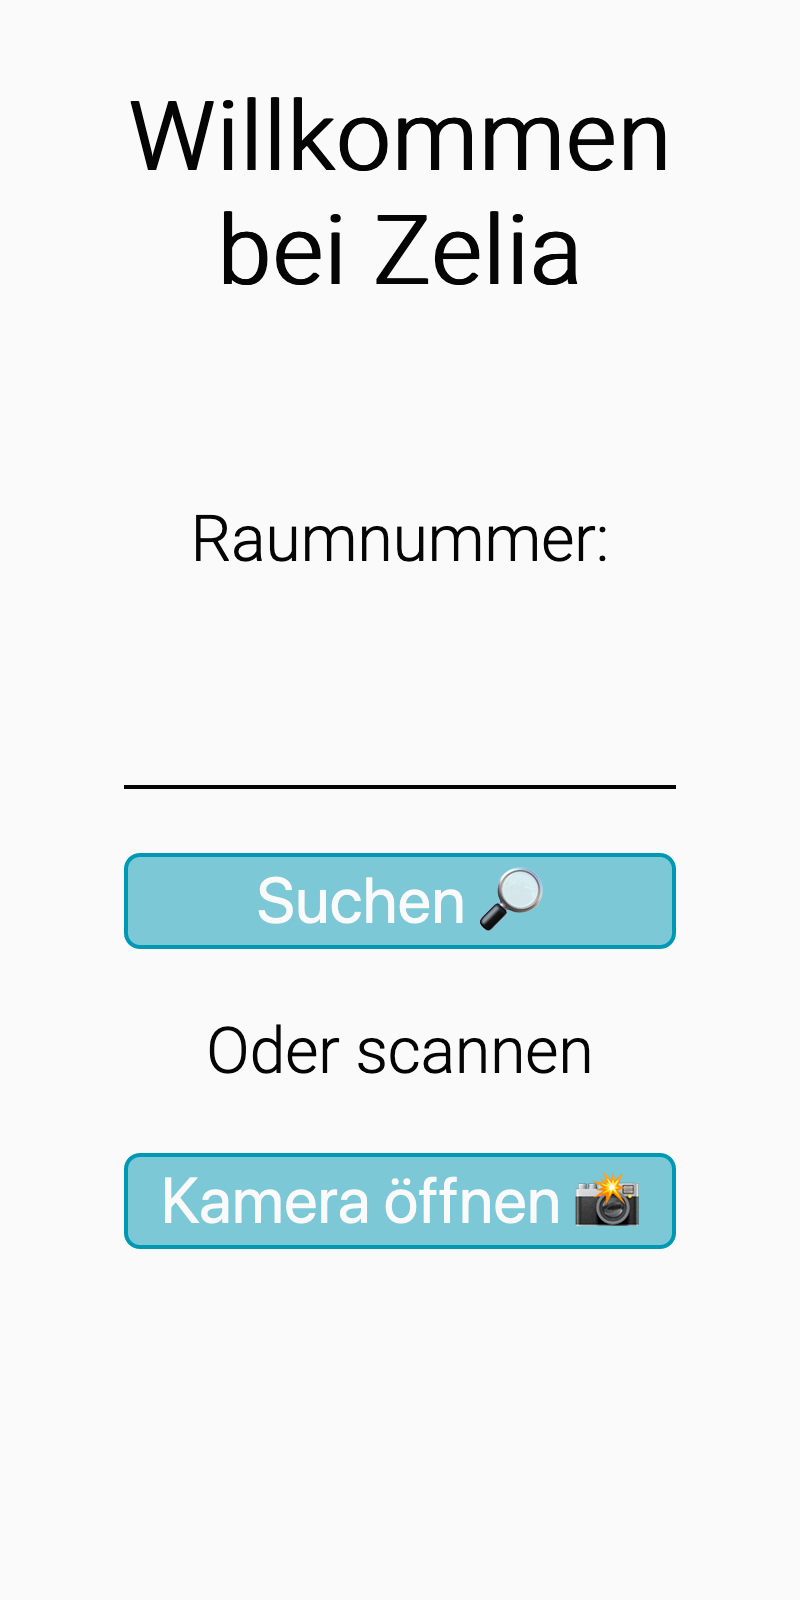
\includegraphics[height=90mm]{media/Handbuch/zelia_start.png}
    \caption{Startseite auf Mobilgeräten}
    \label{fig:zeliastart}
\end{figure}

Auf dieser Startseite hat man die Möglichkeit, eine Raumnummer einzugeben oder einzuscannen, um auf die Rauminformationsseite zu gelangen. Wie im Kapitel \ref{sec:webcompstart} beschrieben, bekommt man anhand der manuellen Eingabe Vorschläge, welche Räume es gibt (siehe Abbildung \ref{fig:compinput}, Kapitel "Die Startseite" \ref{sec:webcompstart}, Seite \pageref{sec:webcompstart}). 

Die Rauminformationsseite zeigt zum einen Daten über einen Raum an wie Anzahl an Plätzen oder Computern und zum anderen den aktuellen Stundenplan. Mit dem "Home"-Link kann man auf die Startseite zurückkehren. Die Emojis zeigen auf einen Blick, was in diesem Raum möglich ist. Zum Beispiel, ob der Raum für Rollstuhlfahrer*innen geeignet ist oder ob ein Waschbecken vorhanden ist. Wenn man auf diese Emojis drückt, klappt eine Auflistung auf, in der eine genauere Beschreibung des Raumes steht.

\begin{figure}[H]
    \centering
    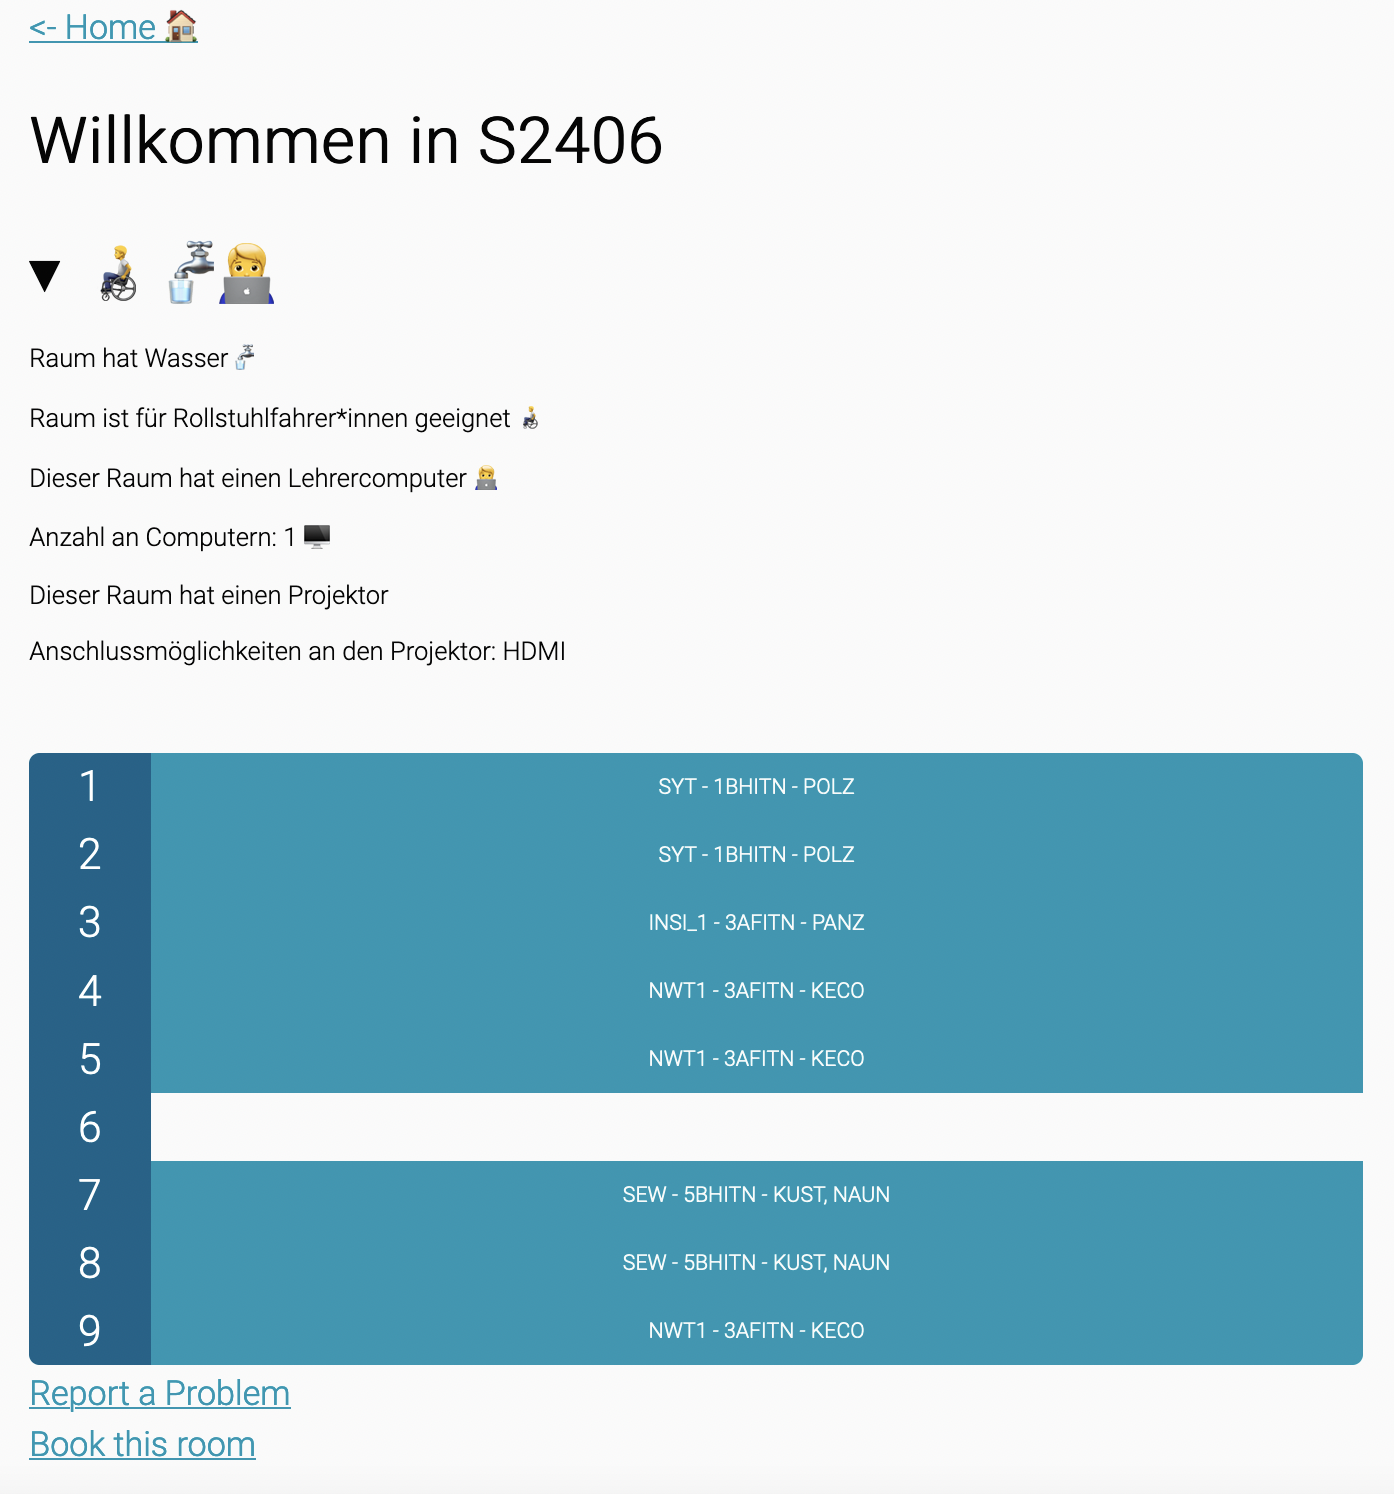
\includegraphics[width=120mm]{media/WebComponents/Rauminformationsseite.png}
    \caption{Informationsseite auf Computern}
    \label{fig:zeliainfopage}
\end{figure}

Ganz unten auf der \ZELIA\ Informationsseite sind zwei Links mit den Namen "Raum melden" und "Raum buchen", über die man auf die jeweilige Raumbuchungs- oder Raummeldungsseite gelangt. Diese beiden Seiten sind ähnlich aufgebaut. Sie bestehen aus einem Formular, um die Daten anzugeben, die notwendig sind. Meldungs- und Buchungsvorgänge kann man mit Links, die auf die Übersichtsseite zurückführen, abbrechen.

\begin{figure}[H]
    \centering
    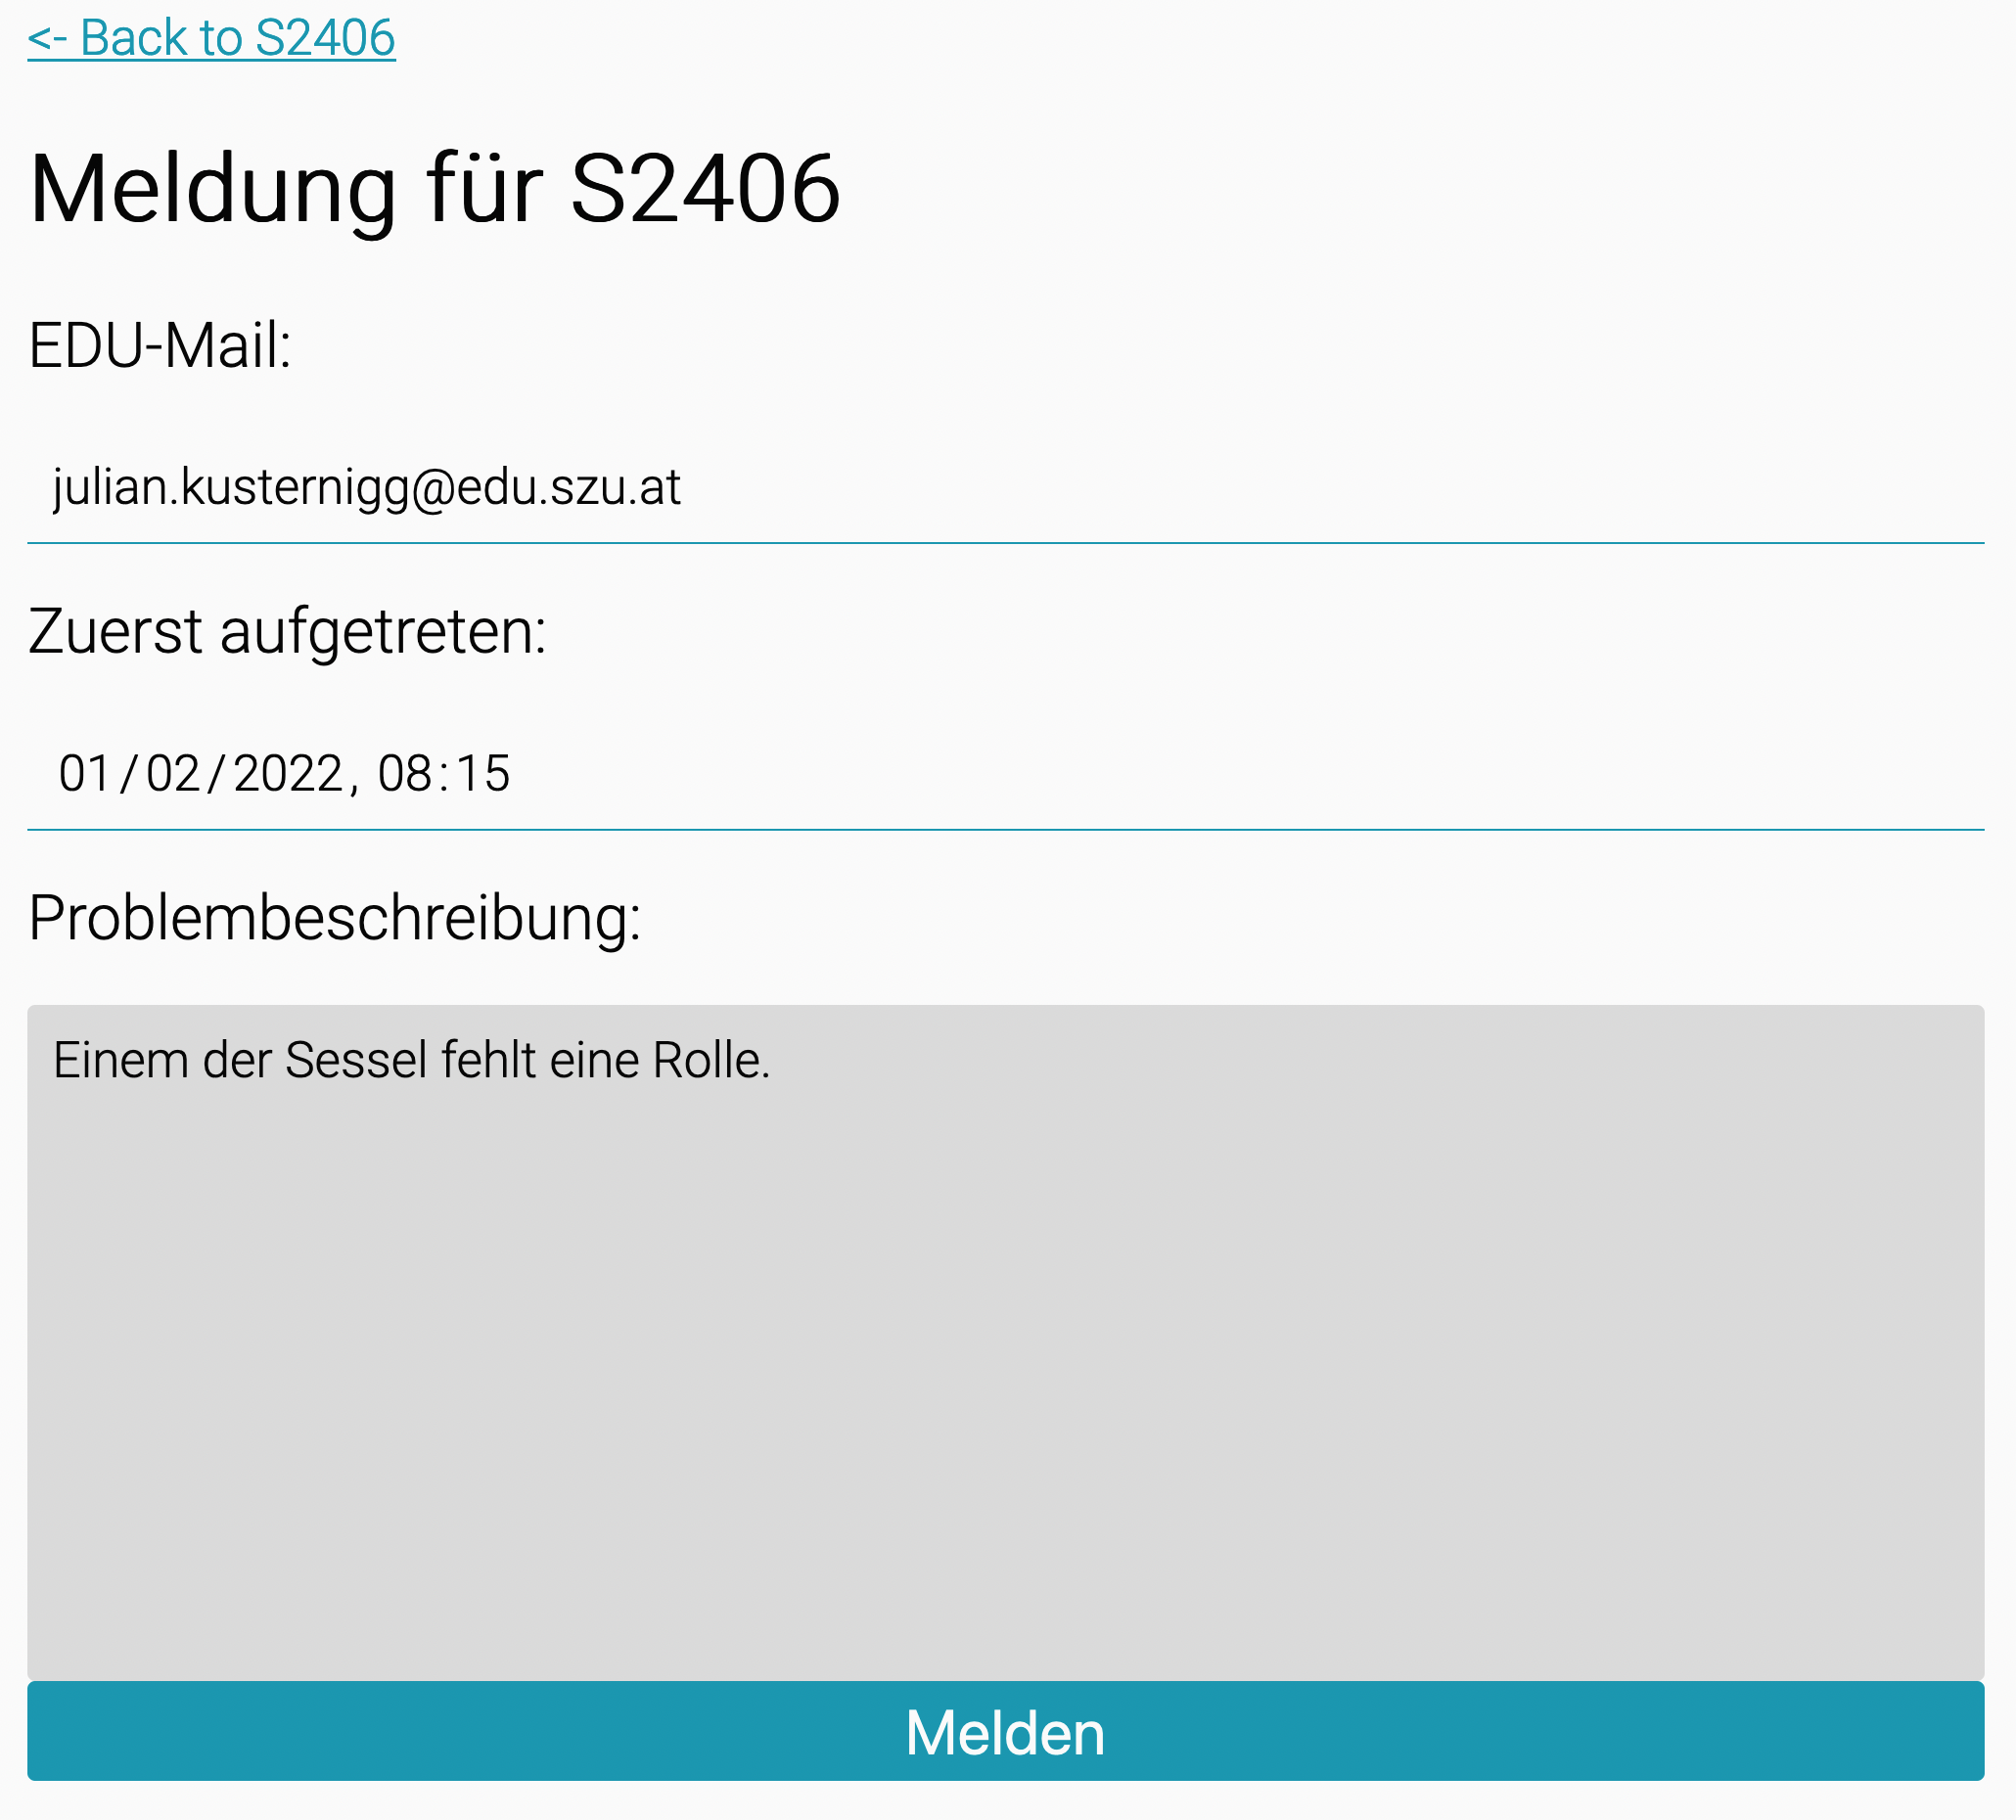
\includegraphics[width=80mm]{media/WebComponents/Meldungsseite_light.png}
    \caption{Meldungsseite}
    
\end{figure}

\begin{figure}[H]
    \centering
    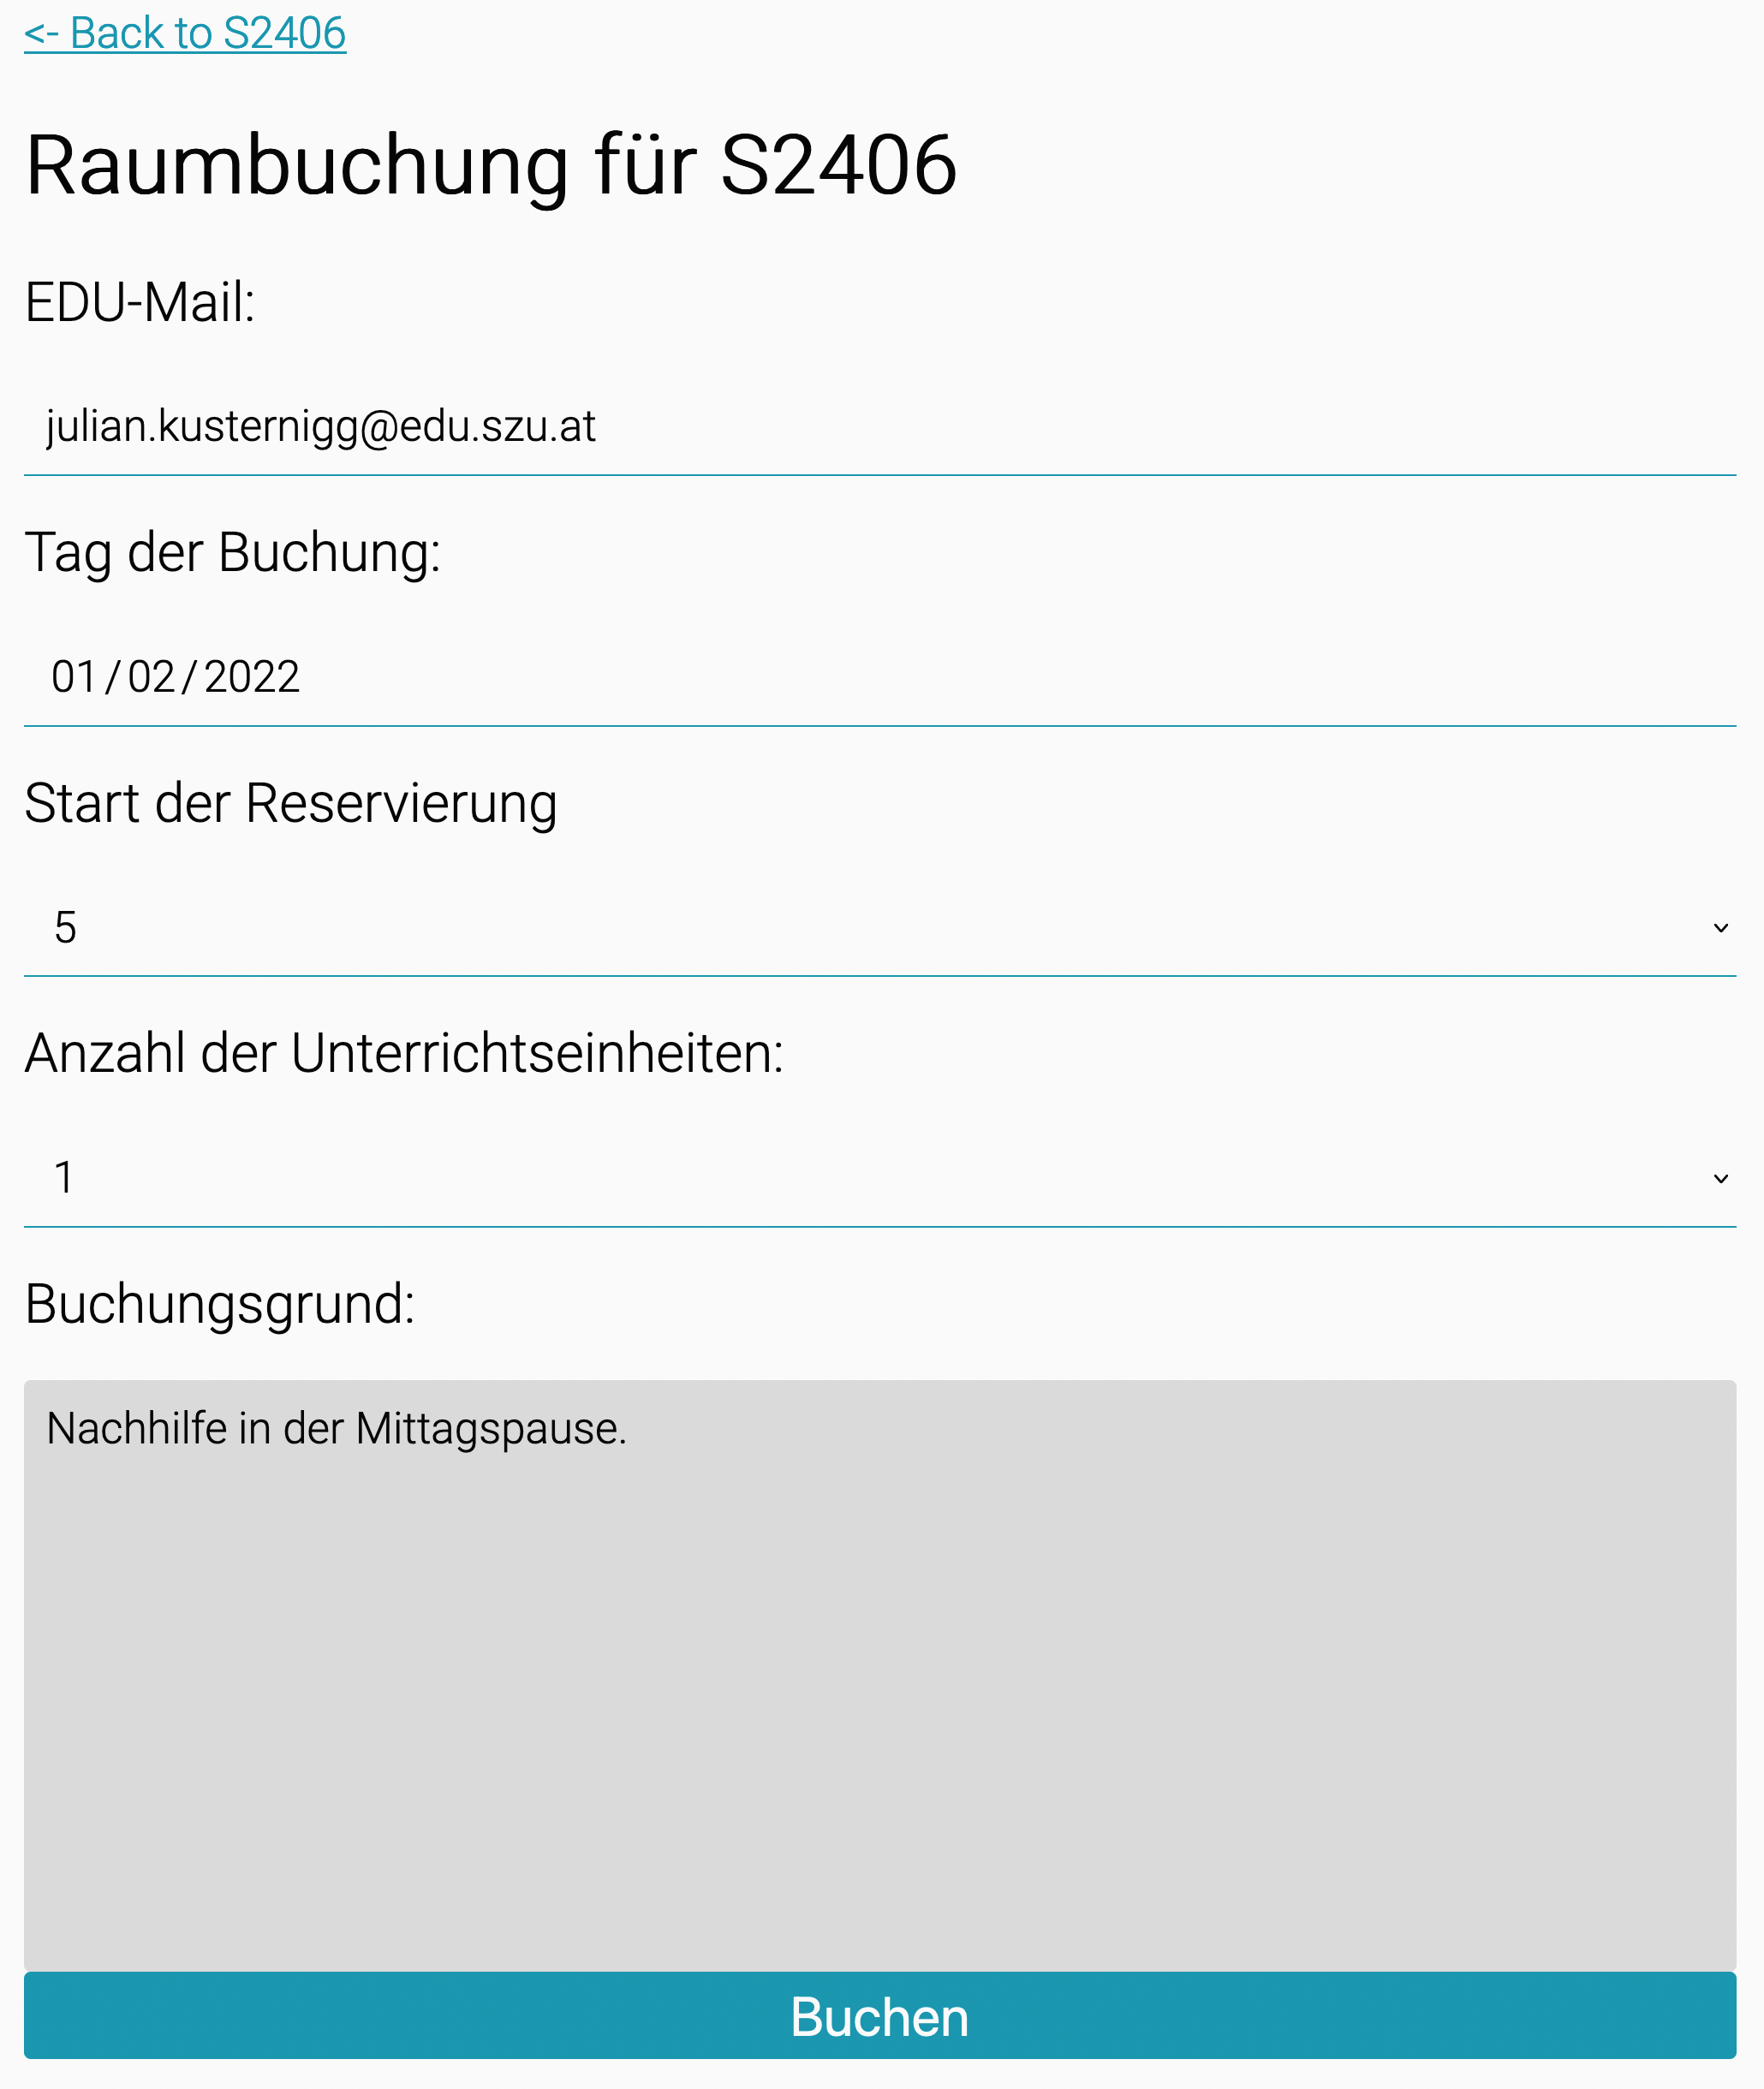
\includegraphics[width=80mm]{media/WebComponents/Buchungsseite_light.png}
    \caption{Buchungsseite}
\end{figure}

Nachdem man das Formular abgeschickt hat und die Meldung oder Buchung mit dem Link aus der Bestätigungsmail verifiziert wurde, können Lehrer*innen die angegebenen Daten in der Adminübersicht sehen.

\hthree{Verwendung für Administrator*innen}

Lehrer*innen mit Administartorbenutzern können die Meldungen und Buchungen ihrer zugeordneten Klassenräume ansehen und abarbeiten. Dafür müssen sie den Pfad \emph{/admin} manuell in die Suchleiste eingeben. Auf dieser Seite befindet sich ein Anmeldeformular. In dieses muss der jeweilige Administrator gültige Zugangsdaten eingeben, welche vom \ZELIA-Administrator vergeben werden. 

\begin{figure}[H]
    \centering
    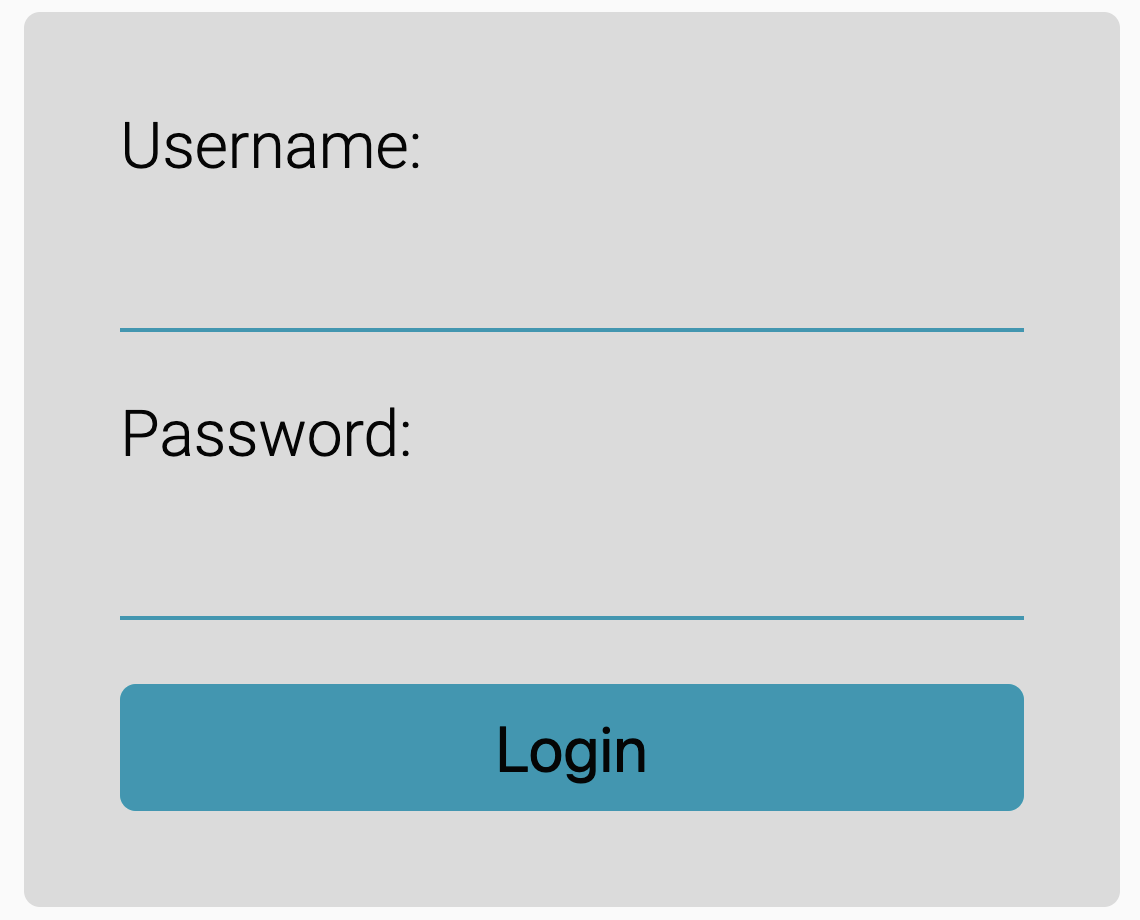
\includegraphics[width=80mm]{media/WebComponents/Login_light.png}
    \caption{Admin Anmeldeformular}
\end{figure}

Nachdem die Anmeldung erfolgreich war, sieht man die Adminübersicht, auch "Admin Dashboard" genannt.

\begin{figure}[H]
    \centering
    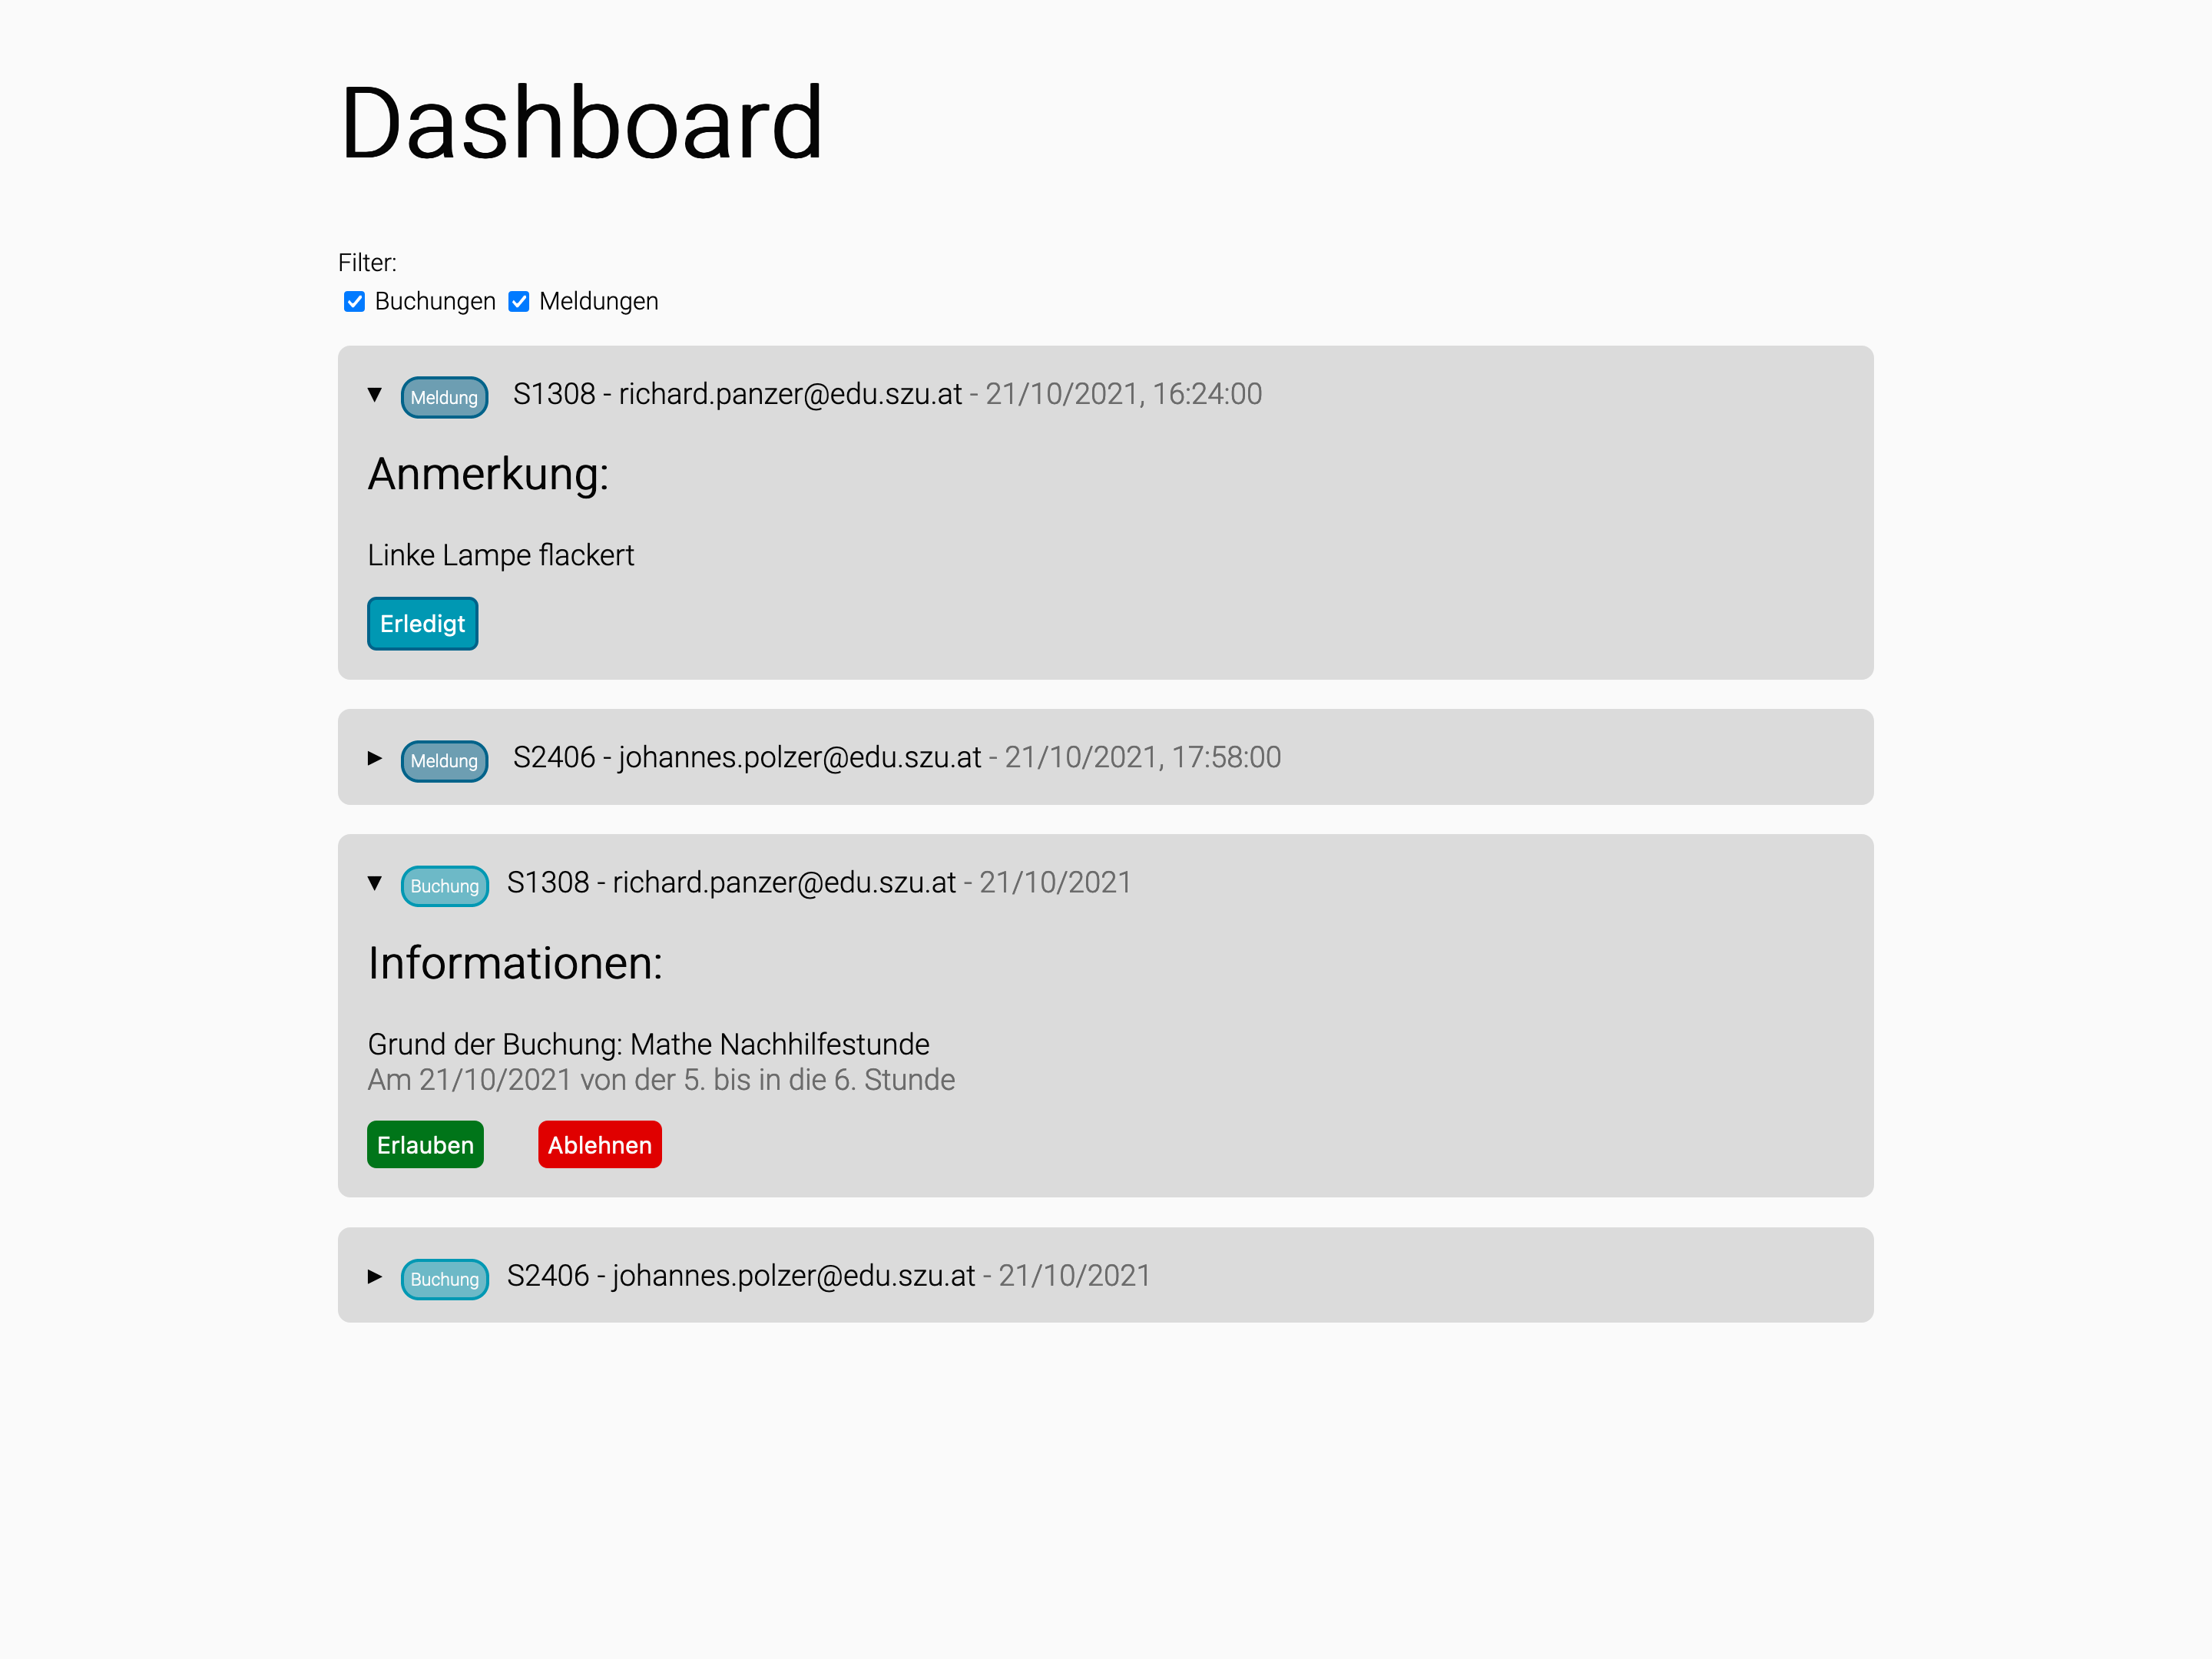
\includegraphics[width=120mm]{media/WebComponents/AdminSeite_light.png}
    \caption{Adminübersicht auf Computern}
\end{figure}

Hier können Meldungen über Defekte im Raum abgearbeitet und Buchungsanfragen akzeptiert oder abgelehnt werden.
Für mehr Details über das "Admin Dashboard", siehe Kapitel "Admin Login" und "Dashboard" \ref{sec:webcomplogdash}.
